%% For distribution of the original source see the terms
%% for copying and modification in the file samples.dtx.
%% 
%% This generated file may be distributed as long as the
%% original source files, as listed above, are part of the
%% same distribution. (The sources need not necessarily be
%% in the same archive or directory.)
%%
%%
%% Commands for TeXCount
%TC:macro \cite [option:text,text]
%TC:macro \citep [option:text,text]
%TC:macro \citet [option:text,text]
%TC:envir table 0 1
%TC:envir table* 0 1
%TC:envir tabular [ignore] word
%TC:envir displaymath 0 word
%TC:envir math 0 word
%TC:envir comment 0 0
%%
%%
%% For submission and review of your manuscript please change the
%% command to \documentclass[manuscript, screen, review]{acmart}.
%%
%% When submitting camera ready or to TAPS, please change the command
%% to \documentclass[sigconf]{acmart} or whichever template is required
%% for your publication.
%%
%%
\documentclass[acmsmall, review, screen]{acmart}

%%
%% \BibTeX command to typeset BibTeX logo in the docs
\AtBeginDocument{%
  \providecommand\BibTeX{{%
    Bib\TeX}}}

%% Rights management information.  This information is sent to you
%% when you complete the rights form.  These commands have SAMPLE
%% values in them; it is your responsibility as an author to replace
%% the commands and values with those provided to you when you
%% complete the rights form.
\setcopyright{acmcopyright}
\copyrightyear{2022}
\acmYear{2022}
\acmDOI{XXXXXXX.XXXXXXX}

%% These commands are for a PROCEEDINGS abstract or paper.
\acmConference[Conference acronym 'XX]{Make sure to enter the correct
  conference title from your rights confirmation emai}{June 03--05,
  2018}{Woodstock, NY}
%%
%%  Uncomment \acmBooktitle if the title of the proceedings is different
%%  from ``Proceedings of ...''!
%%
%%\acmBooktitle{Woodstock '18: ACM Symposium on Neural Gaze Detection,
%%  June 03--05, 2018, Woodstock, NY}
\acmPrice{15.00}
\acmISBN{978-1-4503-XXXX-X/18/06}


%%
%% Submission ID.
%% Use this when submitting an article to a sponsored event. You'll
%% receive a unique submission ID from the organizers
%% of the event, and this ID should be used as the parameter to this command.
%%\acmSubmissionID{123-A56-BU3}

%%
%% For managing citations, it is recommended to use bibliography
%% files in BibTeX format.
%%
%% You can then either use BibTeX with the ACM-Reference-Format style,
%% or BibLaTeX with the acmnumeric or acmauthoryear sytles, that include
%% support for advanced citation of software artefact from the
%% biblatex-software package, also separately available on CTAN.
%%
%% Look at the sample-*-biblatex.tex files for templates showcasing
%% the biblatex styles.
%%

%%
%% The majority of ACM publications use numbered citations and
%% references.  The command \citestyle{authoryear} switches to the
%% "author year" style.
%%
%% If you are preparing content for an event
%% sponsored by ACM SIGGRAPH, you must use the "author year" style of
%% citations and references.
%% Uncommenting
%% the next command will enable that style.
%%\citestyle{acmauthoryear}

%% Packages
\usepackage{xcolor}
\usepackage{color}
\usepackage{listings}

%% Custom Definitions
\graphicspath{{graph/}}
\definecolor{ForestGreen}{HTML}{009B55}

\lstset{inputpath=code_examples/lib/Examples}
\lstset{
  frame=none,
  xleftmargin=2pt,
  stepnumber=1,
  numbers=left,
  numbersep=5pt,
  numberstyle=\ttfamily\tiny\color[gray]{0.3},
  belowcaptionskip=\bigskipamount,
  escapeinside={*'}{'*},
  language=haskell,
  tabsize=2,
  emphstyle={\bf},
  commentstyle=\color{ForestGreen},
  stringstyle=\mdseries\rmfamily,
  showspaces=false,
  keywordstyle=\bfseries\rmfamily,
  columns=flexible,
  basicstyle=\small\sffamily,
  showstringspaces=false,
  morecomment=[l]\%,
}

% Shorthand command for Lark
\newcommand{\Lark}[0]{\textsc{Lark}}

%% CUSTOM PACKAGES - NON-ACCEPTED
\usepackage{todonotes}

%%
%% end of the preamble, start of the body of the document source.
\begin{document}

\title[Layered Types]{Layered Types -- A structured approach to arbitrarily combine Type Systems}

%%
%% The "author" command and its associated commands are used to define
%% the authors and their affiliations.
%% Of note is the shared affiliation of the first two authors, and the
%% "authornote" and "authornotemark" commands
%% used to denote shared contribution to the research.
\author{Lukas Abelt}
\email{l.abelt@luabelt.de}
\orcid{1234-5678-9012}
\affiliation{%
  \institution{LASIGE}
  \streetaddress{XXX}
  \city{Lisbon}
  \state{}
  \country{Portugal}
  \postcode{}
}

%%
%% The abstract is a short summary of the work to be presented in the
%% article.
\begin{abstract}
	\todo[inline]{TODO: Abstract}
\end{abstract}

%%
%% The code below is generated by the tool at http://dl.acm.org/ccs.cfm.
%% Please copy and paste the code instead of the example below.
\begin{CCSXML}
\end{CCSXML}
%\ccsdesc[500]{Computer systems organization~Embedded systems}
%\ccsdesc[300]{Computer systems organization~Redundancy}
%\ccsdesc{Computer systems organization~Robotics}
%\ccsdesc[100]{Networks~Network reliability}

%%
%% Keywords. The author(s) should pick words that accurately describe
%% the work being presented. Separate the keywords with commas.
%TODO: Keywords
\keywords{}
%% A "teaser" image appears between the author and affiliation
%% information and the body of the document, and typically spans the
%% page.
\begin{teaserfigure}
  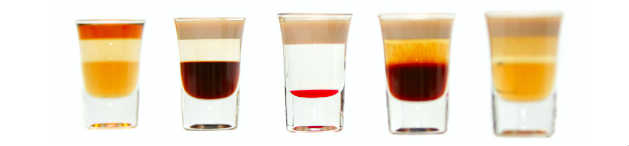
\includegraphics[width=\textwidth]{layered-shots.jpg}
  \label{fig:teaser}
  \caption{Layers in Liquids}
\end{teaserfigure}

\received{20 February 2007}
\received[revised]{12 March 2009}
\received[accepted]{5 June 2009}

%%
%% This command processes the author and affiliation and title
%% information and builds the first part of the formatted document.
\maketitle
\section{Introduction}
\label{sec:introduction}
\subsection{Context}
\label{ssec:context}
Type systems are a core part of most modern programming languages. Most programmers will be familiar with the concept of simple static type systems as they are present in languages such as C++, Java, Rust or Haskell, that assign types to variables and functions and checks that types are used in a correct way. Using static type systems bears a lot of benefits as it can already prevent a multitude of runtime errors.

However, static type systems alone cannot prevent runtime errors alone as they do not present strong enough guarantees. Therefore many other type systems have been proposed over the years. One example of this are \textit{Refinement Types}, also referred to as \textit{Liquid Types}. These allow us to annotate the traditional type system with additional logical predicates in order to ensure semantic properties, which can be checked statically at compile time. Using these techniques also allows us to define pre- and post-conditions on functions' arguments and return values. By properly defining these contracts a developer can clearly communicate and moreover enforce how other developers' code is allowed to interface with their implementations. Examples for constraints might include any of the following:

\begin{itemize}
	\item Ensuring values are in certain bounds
	\item Ensuring that a list is non-empty
	\item Ensuring that data structures certain to specific semantic properties e.g. that they are sorted
\end{itemize}

All in all, refinement types are valuable building blocks to creating reliable software systems. Using them can minimize the risk of any unhandled run-time errors occuring which might lead to undesired or even undefined behavior.

Refinement Types are but one example of the many different typesystems that have been introduced over the years. In this paper we want to discuss how it is possible to combine different type systems and combine their advantages.

\subsection{Motivation}
\label{ssec:motivation}

While various type systems have been proposed over the years, using even one of them in an existing program is not a trivial task. In order to use these more advanced type systems, programmers often depend on specialized tools such as separate type checkers or compilers. Depending on the specific implementation these tools may or may not be easily integratable into existing development workflows. It gets even more complicated when trying to combine multiple type systems. In order to use multiple type systems, programmers then rely on a multitude of different tools that often cannot be arbitrarily combined. This can lead to a lot of overhead and complexity in the development process.

Our motivation for this paper was to propose an approach, that allows to easily extend and combine existing type systems, with the goal of making them more accessible to programmers. We want to achieve this by providing a framework that allows to easily combine different type systems and ensures a consistent type checking process.

The original motivation for this paper however, stems from a problem often prevalent while using refinement types; While Refinement Types vastly imrpove traditional type systems, current implementations still expose some drawbacks in their practical usage. One of these challenges stems from the fact that during the static analysis, each refinement is treated as a single monolithic requirement that needs to be fulfilled. However in reality, a refinement might combine different properties of a type that may benefit from being treated individually.

One example for such a refinement in LiquidHaskell is shown in \Cref{lst:combined_lt}. There, we define a function that extracts the maximum value of a (descendingly) ordered, non-empty list. In this example, this operation is equivalent to simply extracting the \texttt{head} of a list. While we only define one refinement, it actually operates on two different properties of a list. First, it imposes a restriction on it's \texttt{size} by requiring it to be non-empty, while the second restriction imposes an order on the list elements.

\lstinputlisting[firstline=6,caption={Example for a function with a combined Refinement Type in LiquidHaskell},label={lst:combined_lt}]{CombinedLT.hs}

While the refinement concerns two different aspects of the list that are independent from each other, current static analysis implementations of Liquid Types will treat it only as a single combined requirement to be fulfilled. However especially developers could benefit from a system that treats them independently: When writing code that interfaces with already existing codes such a separated approach may give a developer more fine-grained information on which requirements they still need to fulfill in their implementation.

Effectively one could treat such different requirements as separate \textit{Layers} that can be verified independently. Additionally with a proper implementation using such layers may also result in an implementation benefit, that different Layers can be defined individually and combined arbitrarily, as opposed to the example in Listing \Cref{lst:combined_lt} where the combination of the two traits had to be explicitly defined as an refinement on it's own.

One other possible usage of such an iterative approach is that it could allow to more flexibly add different static analysis approaches on top of each other. For example \cite{liquidate-assets} have shown how to use liquid types in Haskell to statically perform cost analysis of different resources such as memory consumption or computational complexity. In their approach they showed that liquid types can be used to reason about their upper and lower bounds. However, in their work they only analysed one resource at a time. However, using a layered approach would allow to easily combine these different resource analyses to eg. track and reason about both memory usage and computational complexity.

\subsection{Problem Definition}
\label{ssec:problem_definition}

Current verification approaches usually focus on verifying a single property of a program at a time. However, in practice, one might needs to verify different properties of the program for different purposes. In current implementations, it is not trivially possible to combine these different verification passes. One specific examplefor this can be found when looking at current implemetnations of Liquid Types. In these, one can only define one liquid type for variables, arguments or return types. This forces us to combine all properties we want to statically check and verify into one joint predicate. Using such an approach has the drawback that all properties are checked simultaneously which might make it difficult for a developer to identify due to which property a type error occurs. Additionally previously declared liquid types may not be reused when wanting to refine them further.

With this paper, we therefore propose a new incremental verification approach that we will refer to as \textit{Layered Types}. The goal of this approach is it for a program to be possible to define individual layers for the verification process that are verified individually. By defining dependencies between those layers, it is possible to define a verification order that ensures that all layers are verified in the correct order. This allows us to define different properties of a program that can be verified independently from each other.

With this paper, we want to tackle the following research questions:

\begin{enumerate}
	\item RQ1: Can we define a layered type system that allows to treat different properties of a program independently from each other?
	\item RQ2: Can we use such a layered type system to improve challenges that are present in current Liquid Type implementations?
\end{enumerate}

While in this paper, we will focus on specific Use-Cases that aim towards using it with Liquid Types, we believe that the proposed approach can be applied to other verification techniques as well. For example, we believe that the proposed approach can be extended to verify all sorts of different properties and typesystems such as e.g. \textit{Linear Types} \cite{linear_types} or \textit{Dependent Types} \cite{dependent_types}.

We also want to make an important distinction on the terminology used within the scope of this paper: While on first glance this approach could be described as an approach to \textit{Gradual Verification}, we will explicitly refer to our approach as \textit{Layered} to distinguish it from \textit{Gradual Verification} techniques. While the latter deal with the gradient between incomplete and complete information (in that case on types), our approach is rather concerned not with what information is available on the typing but rather how it is processed. However, we believe that our approach can also be used to implement gradual verification techniques.

\subsection{Impact}
\label{ssec:impact}

The main impact of this paper is to showcase an approach of how different, dependent or independent, type systems can be combined using a single framework without the need to rely on multiple different tools. This allows to combine the advantages of different type systems and allows to use them in a more flexible way. Additionally, we believe that this approach can be used to improve the usability of Liquid Types and other verification techniques. Specifically, we believe our approach has the potential to have the following impacts on Liquid Types in practice:

\paragraph{Improved Error Messages}

One current challenge when using liquid types is that all predicates for a type are checked simultaneously. This can make it difficult to identify which predicate caused a type liquid error. By separating the predicates into separate \textit{Layers} and verifying them individually, it is possible to precisely identify the predicate causing the type error. We expect this to help developers to more easily identify and fix these type errors in their code.

\paragraph{Improved Usability and Reusability}

In current Liquid Type implementations, types that require multiple predicates are defined as a single type. This may make it difficult for a developer to directly identify which properties a specific liquid type ensures. By separating different properties into a more fine-grained layered approach, this may make it easier to identify these properties. Additionally, by separating the predicates into different layers, it is possible to reuse liquid types in a more flexible way. For example, if a developer wants to refine a previously defined liquid type, they can now do so by adding a new layer to it, instead of having to redefine the entire type.

\paragraph{Improved Composability}

In addition to the improved reusability of our approach, we also expect it to improve the composability of different liquid types. With our suggested approach, new refinements can simply be created by composing already existing layers. This vastly increases modularity of the liquid type approach. It also may allow to re-use layers that have already been defined by other developers for ones own implementation.

\paragraph{Improved Modularity}

By separating the predicates into different layers, it is possible to reuse previously defined liquid types in a more flexible way. For example, if a developer wants to refine a previously defined liquid type, they can now do so by adding a new layer to it, instead of having to redefine the entire type. Additionally, this also supports the seperation of concerns when collaborating with other developers. In current implementations, when interfacing with other developers' code, one needs to be aware of all the refinements required by such code in order to interact with it. When different properties are divided into proper layers, this is no longer required.

\subsection{Approach}
\label{ssec:approach}

We will start by giving a brief overview of the general principles of refinement types and liquid types in general in section \ref{sec:background}. Additionally, we will discuss the current state of the art in liquid types and gradual verification in section \ref{sec:related}. 

In section \ref{sec:implementation} we will first give a more detailed description of our approach and define a simple functional language that we will use for further demonstration. We will then describe in detail the proposed architecture of our layered type checker and our layered verification framework.

In section \ref{sec:use_cases} we will present two specific use cases. One of which will showcase a way of combining different independent type systems using our layered approach. The other use case will showcase how our approach can be used to verify different properties independently in a liquid type system.

In section \ref{sec:evaluation} we will discuss the limitations of our approach and possible extensions. Additionally, we will evaluate how our approach compares to using a pure, non-layered, verification approach.

\subsection{Contributions}
\label{ssec:contributions}

With this paper we deliver the following contributions:

\begin{enumerate}
	\item We propose a new approach to incremental verification that we will refer to as \textit{Layered Types}.
	\item We present an architecture for a layered verification framework that allows to verify different properties of a program independently from each other.
	\item We present two specific use cases that showcase how our approach can be used to verify different properties independently in a liquid type system.
	\item We deliver a prototype implementation of our layered type checker framework, including some example implementations for layers in said framework. Our implementation is available at \url{https://www.github.com/LuAbelt/LayeredTypes}.
\end{enumerate}


\section{Background}
\label{sec:background}

\subsection{Type Systems}
\subsection{Liquid Types}




\section{Related Work}
\label{sec:related}



\section{Implementation}
\label{sec:implementation}

In this section we will describe our implementation of a layered typing approach in detail. We will start by describing the simple functional language we will use for our examples. We will then describe how our layered type checker is implemented. Finally, we will showcase how our approach can be used on various simple examples.

\subsection{Language}
\label{ssec:language}

To demonstrate our layered approach we implemented a simple functional language. The syntax of said language is described in Fig. \ref{fig:lang}. The language is similar to most simple functional languages. Implicitly, our language natively supports \texttt{Boolean} and \texttt{Integer} datatypes through the available constants. However, the language on it's own does not require any type annotations.

\begin{figure}[ht!]
\begin{align*}
	id \in \texttt{Ident}\ 	&::=\ [a...zA...Z]+ \\
	v \in \texttt{Var}\ 	&::=\ id \\
	f \in \texttt{Fun}\ 	&::=\ id_1\ ...\ id_n\ \{\ s\ \}\\
	e \in \texttt{Expr}\ 	&::=\ v\ |\ c\ |\ (\ e\ \circledplus\ e\ )\ |\ (e\ \circleddot\ e)\ |\ f(e)\ |\ f(e_1,\ ...,\ e_n)  \\
	\texttt{CustomExpr}\ 	&::=\ \texttt{String}\\
	c \in \texttt{Const}\ 	&::=\ \texttt{True}\ |\ \texttt{False}\ |\ \mathbb{Z} \\
	\texttt{Assign}\ 	&::=\ v\ :=\ e\ |\ v\ :=\ \texttt{CustomExpr}\ \\
	s \in \texttt{Stmt}\ 	&::=\ \texttt{Assign}\ |\ \texttt{if}\ v\ \texttt{then}\ \lbrace\ s_1\ \rbrace\ \texttt{else}\ \lbrace\ s_2\ \rbrace\ |\ \texttt{let}\ v\ :=\ e\ \texttt{in}\ \lbrace\ s\ \rbrace\ |\ \ell\ |\ s_1\ s_2\ \\
	\ell \in \texttt{Layer}\ 	&::=\ id_1::id_2::\texttt{String} \\
	\circledplus\ 		&::=\ \texttt{+}\ |\ \texttt{-} \\
	\circleddot\ 		&::=\ \texttt{!=}\ |\ \texttt{==}\ |\ \texttt{<} \ |\ \texttt{>} \ |\ \texttt{<=} \ |\ \texttt{>=} \\
\end{align*}
\caption{Syntax of the simple functional language}
\label{fig:lang}
\end{figure}

While our language allows to define functions on its own, we will further allow the usage of function names that may have not been defined in the language itself. To allow this, the user can create a separate Python file that contains the definitions of additional functions. Our interpreter will then forward the calls to these functions to the Python interpreter. This allows us to easily access more complicated functionality such as the \texttt{print} function.

Additionally to standard operations, the syntax of the language supports creating layers that can be applied onto each identifier. The syntax of a layer consists of the following:
\begin{itemize}
	\item $id_1$ -- The name of the identifier to be refined
	\item $id_2$ -- The name of the layer
	\item An arbitrary \textit{String} that represents the refinement. Note that the syntax does not restrict the format of this string, as this information will be parsed later by the corresponding type checking layer.
\end{itemize}

These layers can be used to define properties. Depending on the specific implementation of a layer, these properties can apply to identifiers or can be used to define properties of the type system the layer defines. In a very basic and minimal approach these layers can be used to annotate types to variables and functions. Additionally, one might add additional layers to a variable to ensure more properties. Each layer will be checked individually and independently. A more detailled approach of the architecture behind our layered approach will be described in section \ref{ssec:architecture}.

An example how a program written in our language could look like can be seen in \ref{lst:fac_example}. The program defines a factorial function that is refined in two layers. The first layer \textit{base} is a simple type layer that defines that \texttt{fac} takes an \texttt{Int} and returns an \texttt{Int}. The second layer \textit{liquid} is a refinement layer that refines that the input should be greater or equal to zero and that the output will be greater than zero. The implementations of the \textit{base} and \textit{liquid} layer are not part of our language and have to be implemented independently.

\begin{lstlisting}[caption={Example of a factorial function in our simple language}, label={lst:fac_example}]
fac::base:: Int -> Int
fac::liquid:: {v:Int | v >= 0} -> {v:Int | v > 0}
fac x { 
let cond := (x == 0) in
	if cond then 
		1 
	else 
		x * fac (x - 1) 
}
\end{lstlisting}

\subsection{Language Implementation Architecture}
\label{ssec:architecture}

The implementation of our language will be done in the \texttt{Python} programming language. Generally the implementation can be divided into three individual parts, which we will describe throughout this section:

\begin{enumerate}
	\item A parser that parses the input program and creates an abstract syntax tree (AST) of the program.
	\item A layered type checker that checks the defined type layers for the tree incrementally.
	\item An interpreter that executes the program.
\end{enumerate}

To parse a input program, we will use the Python library \Lark{} \cite{Lark}. This library allows us to define a grammar for the language and then parse a program according to this grammar. All further processing will be performed on the resulting AST. To process and execute the AST we will use the Visitors and Transformers provided by the \Lark{} library.

After parsing the AST there are a few simple checks that are run by an initial interpreter pass. Namely, our framework will check that variables are assigned to at least once before they are used in another expression, it will make sure that \texttt{let} does not redeclare an already existing variable. Additionally, function names cannot be defined twice and the framework will also check that functons that are called have either been defined previously in the source file or alternatively are defined externally in Python.

After this initial check has passed, the main part of our work, the layered type checker, will start processing the layers. A "Layer" here refers to a custom implementation that has to be defined in a separate Python file by the user. Based on the defined layer name, our framework will dynamically load the python file as an independent module and will use it to run the type-checker for this layer. Our framework supports the definition of the following functions for each layer:

\begin{itemize}
	\item \texttt{depends\_on} -- This function returns a list of strings. Each string represents a name of a layer that this layer depends on and thus has to be checked before this layer can be run. This is used to ensure that the layers are checked in the correct order.
	\item \texttt{run\_before} -- This function is similar to \texttt{depends\_on} but returns a list of layers that must not run before this layer has been checked corretly. Together with the \texttt{depends\_on} function this allows to flexibly insert layers into any step of the type-checking process.
	\item \texttt{parse\_type} -- This function may be used to define and parse custom data types that are defined usinf the $CustomExpr$ rule in the grammar. \todo[inline]{This is a functionality we discussed in the beginning, that would be nice. However for our current use cases we do not really need it. Should we keep it in the framework or just omit it?}
	\item \texttt{typecheck} -- This function is used to check the layer. It is passed the AST of the program with all the annotated information from the previous layers. It should return the annotated tree with the new layer information added.
\end{itemize}

Using the \texttt{depends\_on} function, the layered type checker will first build a dependency graph of all layers. By using the dependency graph we can calculate the topological order of layers that can be checked in the correct order. Additionally this also allows to check independent layers in parallel. Only if all layers have been checked successfully, the program will be executed.

In order to communicate annotated information between the different layers, we replace the \texttt{Tree} \Lark{} class with our own \texttt{AnnotatedTree} class. This class allows us to store a dictionary of annotations for each node in the tree. The annotations are stored as a dictionary of dictionaries. The first key of the dictionary is the name of the layer, the second key is the name of the annotation. This allows us to store multiple annotations for each layer. The \texttt{AnnotatedTree} class also provides a simple interface to access and add annotations which can be used by developers implementing new layers:

\begin{itemize}
	\item \texttt{get\_layer\_annotation(layer\_id, identifier, key)} -- This function returns the annotation with the given key for the given identifier in the given layer. If no annotation is found, it returns \texttt{None}.
	\item \texttt{get\_all\_layer\_annotations(layer\_id, identifier)} -- This function returns a dictionary of all annotations for the given identifier in the given layer. If no annotations are found, it returns an empty dictionary.
	\item \texttt{add\_layer\_annotation(layer\_id, identifier, key, value)} -- This function adds a annotation with the given key for the given identifier in the given layer to the given value.
	\item \texttt{update\_layer\_annotations(layer\_id, identifier, values)} -- This updates the layer annotations for the given identifier in the given layer with the given dictionary of values.
\end{itemize}

Using this architecture, we provide a flexible framework that allows to easily extend our toy language with different layers that can be used to implement different type systems. Similar to passes in a compiler, the layers can be added and removed easily. Additionally, the layers can be easily combined to create more complex type systems.


\section{Example Use-Cases}
\label{ssec:use_cases}
For the scope of this paper, we have developed two exemplary use-cases for our framework that demonstrates our layered verification approach. In the first use-case, we defined a simple program that uses multiple different, partly independent type systems. For our second example, we use our framework to present a more flexible approach to using Liquid Types.

\subsection{Use Case 1 -- File Processing}
\label{sssec:use_case_1}

In our first use case we implemented a small program that processes the contents of a text file. Througout this section we will describe the program and the implemented layers required to realize this program. Lastly we will discuss the findings and benefits we gained from using our layered verification approach.

\subsubsection{Description}
In our first use-case we design a small program that reads contents from a file and performs certain operations based on that. The base code for our example can be found in Listing \ref{lst:uc1_code}. In our example, the file to be read will contain one number per each line. Depending on whether the number is positive or negative, we add the number as is or the square of the number to the resulting value.

\begin{lstlisting}
processLine lines idx length {
    end := idx == length

    if end then {
        0
    } else {

        curLine := getLine(lines, idx)

        number := strToInt(curLine)

        greaterThanZero := number > 0

        if greaterThanZero then {
            number + processLine(lines, idx + 1, length)
        } else {
            (number * number) + processLine(lines, idx + 1, length)
        }

    }
}

processLines lines {
    length := len(lines)

    idx := 0
    processLine(lines, idx, length)
}

fileName := "numbers.data"
fileHandle := openFile(fileName)
lines := readLines(fileHandle)
closeFile(fileHandle)
total := processLines(lines)

print(total)
total

\end{lstlisting}

All functions that have not been defined directly \ref{lst:uc1_code} are provided in a separate, external python file. As our language on itself does not include a type system and there are no layer annotations in the code above, no type checking will be performed on the code as it is presented.

However even this simple example could already introduce several errors that could be prevented by introducing some static analysis. First of all, it does not provide any information about the variable and function type and thus, we cannot ensure that functions are called with arguments of the correct types which might lead to runtime errors.

Additionally we our code interacts with the file it operates on through a file descriptor. TThis file descriptor can be viewed as a resource that might have an implicit or explicit internal state. In a very simple approach this file descriptor could be in the states "Open" or "Closed". In order to read from it, it should be in an "Open" state and additionally we should ensure that by the end of our program the resource has been properly closed again.

In order to improve our example code and allow static analysis, we therefore will introduce three layers:
\begin{enumerate}
	\item A \textit{Type} Layer -- This layer will be used to simply define variable and function types
	\item The \textit{Typechecking} Layer -- This layer will allow to flexibly define a type system and then use the information provided by the \textit{Type} layer to check if the program is well-typed. It therefore depends on the \textit{Type} layer to provide the type information.
	\item A \textit{State} Layer -- This layer will be used to define states on variables. Additionally it can model state transitions. We will use it to track the state of the file descriptor. This layer operates completely independent from the \textit{Type} and \textit{Typechecking} layer.
\end{enumerate}

\subsubsection{Implemented Layers}
In the following sections we will explain in more detail how the layers are implemented and what Syntax they use.

\paragraph{Types Layer}
The \textit{Types} layer is the first layer that is checked. It is used to define the types of variables and functions. To define the type of a variable we use the \texttt{Layer} syntax of our language. A layer definition for the \textit{Types} layer looks as follows:

\begin{lstlisting}
identifier :: types :: Type
\end{lstlisting}

The \texttt{identifier} is the name of the variable or function for which we want to define the type. The \texttt{types} keyword is used to associate this information with the correct layer. The \texttt{Type} is the desired type information to be annotated. There are no restrictions on how a \texttt{Type} should look, as the types layer simply annotates the given string into the current node and does not further process it. For example to define the type of a variable \texttt{foo} as \texttt{int} we would write:

\begin{lstlisting}
foo :: types :: int
\end{lstlisting}

In order to define the type of a function, there is a slight adaption to this syntax. While the first two parts are identical to the variable definition, we now need to provide type information for each argument of the function. This is done by using the \texttt{Type} syntax for each argument and then separating them with an arrow symbol \texttt{->}. The return type of the function is then defined by the last \texttt{Type}. If a function does not take an argument the defintion simply starts with the arrow symbol. The following code piece contains an example for a function \texttt{f} that takes two arguments of type \texttt{int} and returns a value of type \texttt{bool}, and a function \texttt{g} that does not take any arguments and returns a value of type \texttt{string}:

\begin{lstlisting}
f :: types :: int -> int -> bool
g :: types :: -> string
\end{lstlisting}

It is important to note that the \textit{Types} layer does not perform any type checking. It simply annotates the given type information into the AST. The \textit{Types} layer only checks for the following inconsistencies:

\begin{itemize}
	\item The type for a variable can only be defined once in the current scope.
	\item When encountering a function definition, the type for it needs to be defined before the function signature. Additionally the number of arguments in the function signature needs to match the number of arguments in the type definition.
\end{itemize}

Any further type checking is performed by the \textit{Typechecking} layer.

\paragraph{Typechecking Layer}

The \textit{Typechecking} layer is used to define a type system and then use the information provided by the \textit{Types} layer to check if the program is well-typed. It therefore depends on the \textit{Types} layer to provide the type information. In our implementation of the type checker, we do not impose any restrictions on the specific type system. We rather provide a generic type checking implementation that allows the user to flexibly define their own types and subtype relationships. However, since our language implicitly natively requires specific expressions to be of a number or boolean type, there are implicitly part of our type system.

To define the specific type system, we use the \texttt{Layer} syntax of our language. However, instead of defining layers for identifiers as in the \textit{Types} layer, we reserve a selected set of keywords to define the type system. Depending on the definition provided by the user, the type checker will internally build a type graph that is used to perform the type checking.

The following keywords are reserved and can be used to define parts of the type system:

\begin{itemize}
	\item \texttt{logicalTypes} -- This keyword is used to define a set of logical types. Multiple types can be defined by separating them with a space.
	\item \texttt{numTypes} -- This keyword is used to define a set of numeric types. Multiple types can be defined by separating them with a space.
	\item \texttt{subtype} -- This keyword is used to define a subtype relationship between two or more types. The syntax for a subtype relationship is \texttt{<type1> <: <type2> <: ... <: <typeN>}. The subtype relationship is then defined by the order of the types. The first type is the supertype and the following type is a subtype of the previous type.
\end{itemize}

The following code piece is a short demonstration of a type system containing different logical types, numeric types and subtype relationships:

\begin{lstlisting}
logicalTypes :: typecheck :: bool
numTypes :: typecheck :: int float
subtype :: typecheck :: float <: int
\end{lstlisting}

The type system defined by the user will be used to perform the typechecking. To perform this typecheck the type checker accesses the annotations provided by the \textit{Types} layer. For the case that a type is neither a numeric or logical type and it does not have any subtype relationships, it is not required to explicitly define it in the type system. The type checker will then simply assume the existance of such a type that is not a subtype of any other type nor does it have any subtypes.

Our type checker will perform the following checks:

\begin{itemize}
	\item The type of each variable needs to be defined.
	\item When assigning a value to a variable, the type of the value needs to be a subtype of the type of the variable.
	\item When performing a logical operations (e.g. \texttt{\&\&}, \texttt{||}) the type of the operands needs to be a logical type. The result of the operation will be a logical type.
	\item When performing a numeric operation (e.g. \texttt{+}, \texttt{-}, \texttt{*}, \texttt{/}) the type of the operands needs to be a numeric type. The result of the operation will be the most general numeric type of the operands.
	\item When performing a comparison operation (e.g. \texttt{==}, \texttt{!=}, \texttt{<}, \texttt{>}, \texttt{<=}, \texttt{>=}) the type of the operands needs to be compatible. This means that either the right hand side is a subtype of the left hand side or the left hand side is a subtype of the right hand side. The result of such an operation is always a boolean value.
	\item In an \texttt{if} statement the condition needs to be a logical type.
	\item When performing a function call, the number of arguments needs to match the number of arguments in the function definition. Additionally the type of each argument needs to be a subtype of the type of the corresponding argument in the function definition.
\end{itemize}

Since we require the type of each variable to be defined, this means we require full information about the types of all variables. We do not perform any type inference. This is a deliberate design decision, as we want to keep the language as simple as possible. However, by the design of our language, it would be possible to develop an additional layer that runs after the \textit{Types} layer but before the \textit{Typechecking} layer that performs a type inference based on the incomplete information provided.

\paragraph{State Layer}

The \textit{State} layer is used to define states on variables. Similarly, we can use it to check if a variable has a certain state and define state transitions. This can for example be used to track the state of resources that are used by a program. In our implementation, the state of a variable is completely independent of its type, therefore it does not require any dependencies on the \textit{Types} layer.

The state of a variable is defined by a set of strings. Generally there are two ways to check the state of a variable or transition it's state to a new one. Firstly, we can explicitly do this by using a layer statement of the language. Secondly, we can also impose state requirements on arguments of function calls. Then when passing a variable to a function, the layer will check if the variable has the required state and apply the state transition if there are any.

Similar to the \textit{Types} layer, the \textit{State} layer uses the \texttt{Layer} syntax of the language to define the state of a variable. The first part of the layer statement defines the variable or function name to define a state on, while the second part is simply the layer identifier \texttt{state}. The last part of the layer definition defines the state.

A state definition is enclosed by curly brackets and can contain the following parts:

\begin{itemize}
	\item A state \textit{requirement} -- Imposes a restrition on the current state the variable needs to have. This is simply a string that needs to be part of the current state of the variable.
	\item A state \textit{transition} -- Defines a transition to a new state. Generally a state transition has the form \texttt{<oldState> => <newState>}. However, either the old or new state may be omitted. When omitting the old state, this simply means that something is added to the current state of the variable unconditionally. When omitting the new state, this means that the corresponding state string will be removed from the set of states.
\end{itemize}

For our use-case, we want to track the state of the file descriptor. Specifically, we want to make sure, that the file handle is open before we can read from it. Additionally, we do not want to read from a file handle again once it has already been read. Therefore, we define the states \texttt{Open}, \texttt{Consumed} and \texttt{Closed} and define the appropriate state transistions as seen in Listing \ref{lst:uc1_state}. Additionally, at the end of the program, we want to make sure that the file handle is closed. Therefore, we define a state requirement that the file handle needs to be in the state \texttt{Closed}.

\begin{lstlisting}
createFD :: state :: {} -> { Closed }
openFile :: state :: {Closed => Open} -> {}
readLines :: state :: {Open => Consumed} -> {}
closeFile :: state :: {Consumed => Closed} -> {}

-- State requirement at the end of the program
fileDescriptor :: state :: {Closed}
\end{lstlisting}

The final program with all layer annotations can be found in Listing \ref{lst:uc1_annotated}. With these three layers, we have defined the complete type system for this use-case. Using these three layers we can now ensure the following properties of our program statically:

\begin{itemize}
	\item Our program is type safe. This means that we can be sure that the program will not crash due to type errors.
	\item Using the state layer, we ensure that the file descriptor is handled correctly and is in a closed state at the end of the program.
\end{itemize}

\begin{lstlisting}
-- Type Layer Definitions for externally defined functions
getLine :: types :: [string] -> int -> string
strToInt :: types :: string -> int
len :: types :: [string] -> int
createFD :: types :: string -> FileHandle
openFile :: types :: FileHandle -> void
readLines :: types :: FileHandle -> [string]
closeFile :: types :: FileHandle -> void
print :: types :: Any -> void

-- Layer definitions for type checking
logicalTypes :: typecheck :: bool
numTypes :: typecheck :: int
subtype :: typecheck :: int <: Any
subtype :: typecheck :: string <: Any

-- State layer definitions
createFD :: state :: {} -> { Closed }
openFile :: state :: {Closed => Open} -> {}
readLines :: state :: {Open => Consumed} -> {}
closeFile :: state :: {Consumed => Closed} -> {}

processLine :: types :: [string] -> int -> int -> int
processLine lines idx length {

    end :: types :: bool
    end := idx == length

    if end then {
        0
    } else {

        curLine :: types :: string
        curLine := getLine(lines, idx)

        number :: types :: int
        number := strToInt(curLine)

        greaterThanZero :: types :: bool
        greaterThanZero := number > 0

        if greaterThanZero then {
            number + processLine(lines, idx + 1, length)
        } else {
            (number * number) + processLine(lines, idx + 1, length)
        }

    }
}

processLines :: types :: [string] -> int
processLines lines {
    length :: types :: int
    length := len(lines)

    idx :: types :: int
    idx := 0
    processLine(lines, idx, length)
}

fileName :: types :: string
fileName := "numbers.data"

fileDescriptor :: types :: FileHandle
fileDescriptor := createFD(fileName)

openFile(fileDescriptor)

lines :: types :: [string]
lines := readLines(fileDescriptor)

closeFile(fileDescriptor)

total :: types :: int
total := processLines(lines)

print(total)
total

-- State post-conditions
-- The file handle is closed after the program has finished
fileDescriptor :: state :: {Closed}
\end{lstlisting}

\subsubsection{Discussion}

Implementing this first use-case has given us valuable results and insights on our approach. We have successfully implemented three layers independently from each other, however since the \textit{Typecheck} layer depends on the information provided by the \textit{Types} layer, we successfully demonstrated, that information can be communicated between layers. We have also successfully demonstrated that the layers can be used to define a type system for a program. This means that we can use the layers to define a type system for a program and then use the type checker to check if the program is type safe.

Furthermore, as a result of this use-case, we provide an implementation of a state layer. This layer can be used to define states on variables and functions and to check if a variable has a certain state. Additionally, we can use the state layer to define state transitions. This can be used to track the state of resources that are used by a program. We believe that this layer is suitable for a wide range of applications far beyond the simple demonstration we have shown in this use-case.

One shortcoming of our implementation is that we require that the \textit{Types} layer needs to provide full information on the types of all variables and functions. For a developer it would be much more flexible if it would be possible to only provide partial information and use type-inference to deduce the missing information. However, by the design of our framework extending the example to also support type inference is possible. We could for example add a new layer that runs after the \textit{Types} layer but before the \textit{Typecheck} layer. This layer could then perform type inference and annotate the missing information to the AST. This way the \textit{Typecheck} layer would have all the information it needs to perform the type checking. However for the scope of this paper, we have decided not to implement this feature.

\subsection{Use Case 2 -- Liquid Types}
\label{sssec:use_case_2}



\section{Evaluation}
\label{sec:evaluation}



\section{Conclusion}
\label{sec:conclusion}



\section{Acknowledgments}
\label{sec:acknowledgments}
This work was supported by \textit{Fundação para a Ciência e Tecnologia} (FCT) in the LASIGE Research Unit under the ref. UIDB/00408/2020 and UIDP/00408/2020, by the CMU--Portugal project CAMELOT (LISBOA-01-0247-FEDER-045915), and the RAP project under the reference (EXPL/CCI-COM/1306/2021).

\end{document}
\endinput
%%
%% End of file `sample-acmsmall-conf.tex'.
